\documentclass{scrartcl}

\usepackage{graphicx}
\usepackage[utf8]{inputenc}
\usepackage[T1]{fontenc}
\usepackage{lmodern}
\usepackage[english]{babel}
\usepackage{amsmath}
\usepackage{amsthm}
\usepackage{mathtools}
\usepackage{amssymb}
\usepackage{listings}
\usepackage{xparse}
\usepackage{geometry}
\usepackage{enumerate}
\usepackage{tikz}
\usepackage{stmaryrd}
\usepackage[style=english]{csquotes}
\usepackage[language=english, backend=biber, style=alphabetic, sorting=nyt]{biblatex}

\usetikzlibrary{babel, positioning, shapes.geometric, arrows, arrows.meta}
\addbibresource{bibliography.bib}

\title{Ideas}
\author{Simon Pohmann}

\newcommand{\N}{\mathbb{N}}
\newcommand{\Z}{\mathbb{Z}}
\newcommand{\F}{\mathbb{F}}
\newcommand{\C}{\mathbb{C}}
\newcommand{\I}{\mathbb{I}}
\newcommand{\V}{\mathbb{V}}
\newcommand{\End}{\mathrm{End}}
\newcommand{\proj}{\mathrm{proj}}
\newcommand{\Quot}{\mathrm{Quot}}
\newcommand{\Half}{\mathcal{H}}
\newcommand{\Lattice}{\mathcal{L}}
\renewcommand{\O}{O}

\newcommand\restr[2]{{
    \left.\kern-\nulldelimiterspace
    #1
    \vphantom{\big|}
    \right|_{#2}
}}

\newtheorem{prop}{Proposition}[section]
\newtheorem{theorem}[prop]{Theorem}
\newtheorem{lemma}[prop]{Lemma}
\newtheorem{corollary}[prop]{Corollary}

\theoremstyle{definition}
\newtheorem{problem}[prop]{Problem}
\newtheorem{alg}[prop]{Algorithm}
\newtheorem{definition}[prop]{Definition}
\newtheorem{example}[prop]{Example}
\newtheorem{remark}[prop]{Remark}

\begin{document}

\maketitle

\section{$(d, \epsilon)$-structures}

Let $p$ be a prime.
Consider the category $\mathrm{EC}$ defined by
\begin{align*}
    \mathrm{Ob}(\mathrm{EC}) &:= \{ \text{$E$ elliptic curve over $\F_{p^2}$} \} \\
    \mathrm{Hom}_{\mathrm{EC}}(E, E') &:= \{ \text{$\psi: E \to E'$ isogeny} \}
\end{align*}
Have a functor
\begin{align*}
    \cdot^{(p)}: \mathrm{EC} \ &\to \ \mathrm{EC} \\
    \text{$E$ defined by $y^2 = x^3 + Ax + B$} \ &\mapsto \ \text{$E'$ defined by $y^2 = x^3 + A^p x + B^p$} \\
    \left[ \sum_{i, j} a_{ij} x^i y^j : \sum_{i, j} b_{ij} x^i y^j : \sum_{i, j} c_{ij} x^i y^j \right] \ &\mapsto \ \left[ \sum_{i, j} a_{ij}^p x^i y^j : \sum_{i, j} b_{ij}^p x^i y^j : \sum_{i, j} c_{ij}^p x^i y^j \right]
\end{align*}
and a functor
\begin{align*}
    \hat{\cdot}: \mathrm{EC} \ \to \ \mathrm{EC}^{\mathrm{op}}, \quad E \ \mapsto \ E, \quad \phi \ \mapsto \ \hat{\phi}
\end{align*}
$(d, \epsilon)$-structures and their isogenies are given by the category $\mathrm{ES}_{d, \epsilon}$ defined by
\begin{align*}
    \mathrm{Ob}(\mathrm{ES}) &:= \{ (E, \psi) \ | \ E \in \mathrm{EC}, \ \psi: E \to E^{(p)}, \ \hat{\psi} = \epsilon\psi^{(p)} \} \\
    \mathrm{Hom}_{\mathrm{ES}}((E, \psi), (E', \psi')) &:= \{ \phi: E \to E' \ | \ \psi' \circ \phi = \phi^{(p)} \circ \psi \}
\end{align*}

\section{$j$-invariant and modular polynomials}

Consider the $j$-invariant
\begin{equation*}
    j: \Half \to \C
\end{equation*}
that assigns to a complex elliptic curve given by a lattice $\Lattice\{\tau, 1\}$ its j-invariant $j(\tau)$.
Then it is a fact that for $N \in \N$ the map
\begin{equation*}
    j_N: \Half \to \C, \quad \tau \mapsto j(N\tau)
\end{equation*}
is algebraic over $\C(j)$ and its minimal polynomial is $\Phi_N(X, j)$.
This $\Phi_N$ is called modular polynomial, and we have $\Phi_N \in \mathbb{Q}[X, Y]$ and furthermore $\Phi_N(X, Y) = \Phi_N(Y, X)$.

Furthermore, it holds that
\begin{equation*}
    \Phi_N(j(E), j(E')) = 0
\end{equation*}
for any $E'$ such that there is an $N$-isogeny $E \to E'$ (No idea how to prove that).

We see then that for all primes $p$, have
\begin{equation*}
    \Phi_N(j(E), j(E')) = 0
\end{equation*}
for elliptic curves $E, E'$ defined over $\bar{\F}_p$ such that there is an $N$-isogeny $E \to E'$.

This shows that if we have a $(d, \epsilon)$-structure $(E, \psi)$ then
\begin{equation*}
    \Phi_d(j(E), j(E^{(p)})) = \Phi_d(j(E), j(E)^p) = 0
\end{equation*}
as there is the $d$-isogeny $\psi: E \to E^{(p)}$.

\subsection{Supersingularity Polynomials}
Let $p$ be prime and consider
\begin{equation*}
    K = \F_p(A, B) \quad \text{and} \quad E: z = w^3 + Awz^2 + Bz^3
\end{equation*}
Now consider the local ring $R = K\llbracket t \rrbracket$ and the subring (in fact ideal) $R_t := tR$.
Have
\begin{equation*}
    E(R_t) := E(R) \cap \mathbb{P}_{R_t}^2 = \{ (t, \omega(t)) \ | \ t \in R \}
\end{equation*}
where $\omega \in R_t$.

Now we analyse the group law $*$ on $E(R_t)$ given by
\begin{equation*}
    (u * v, \_) := (u, \omega(u)) +_E (v, \omega(v))
\end{equation*}
As e.g. discussed in Silverman, have
\begin{equation*}
    u * v = F(u, v)
\end{equation*}
where
\begin{align*}
    F &:= -T - S - \frac {2A \lambda(T, S) \nu(T, S) + 3B \lambda(T, S)^2 \nu(T, S)} {1 + A \lambda(T, S)^2 + B \lambda(T, S)^3} \in K\llbracket T, S \rrbracket, \\
    \lambda &:= \frac {\omega(T) - \omega(S)} {T - S} \in K\llbracket T, S \rrbracket, \\
    \nu &:= \omega(T) - \lambda(T, S)T \in K\llbracket T, S \rrbracket
\end{align*}
Note that $F$ is a power series in $T, S$ and so we can evaluate $F(u, v)$ in $R_t$ as for $u, v \in R_t$ have that $|u|_t, |v|_t < 1$ have small $t$-adic valuation, so $F(u, v)$ converges.

\subsection*{Slightly different approach}
Assume $x_1 = x, x_2 = ...$ and
\begin{equation*}
    x_{n + 1} = -x_n - x + \frac {q(x_n) + q(x) + 2yy_n} {(x_n - x)^2}
\end{equation*}
Polynomial division yields
\begin{align*}
    x_{n + 1} =& -x_n - x + x_n + 2x + \frac {(A + x^2)x_n - x^3 + Ax + 2B + 2yy_n} {(x_n - x)^2} \\
    =& x + \frac {(A + x^2)x_n - x^3 + Ax + 2B + 2yy_n} {(x_n - x)^2}
\end{align*}
Substituting $w_n = x_n - x$ yields
\begin{align*}
    w_{n + 1} = \frac {(A + x^2)w_n + 2Ax + 2B + 2yy_n} {w_n^2} = \frac {A + x^2} {w_n} + \frac {2Ax + 2B} {w_n^2} + \frac {2yy_n} {w_n^2}
\end{align*}

\subsection*{Class group approach}
Let $k = \F_p(A, B)$ and $E: y^2 = x^3 + Ax + B$ be the ``universal'' elliptic curve defined over $k$.
Let $K$ be the algebraic closure of $k(E)$.
Now have the commutative diagram
\begin{center}
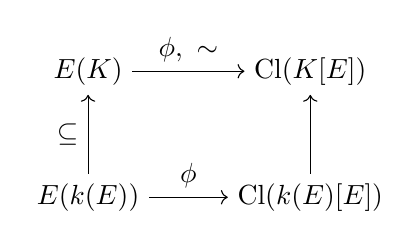
\begin{tikzpicture}
    \node (EkE) {$E(k(E))$};
    \node [above = of EkE] (EK) {$E(K)$};
    \node [right = of EkE] (ClkEE) {$\mathrm{Cl}(k(E)[E])$};
    \node [above = of ClkEE] (ClKE) {$\mathrm{Cl}(K[E])$};
    \draw [->] (EkE) -- (EK) node [midway, left] {$\subseteq$};
    \draw [->] (EK) -- (ClKE) node [midway, above] {$\phi, \ \sim$};
    \draw [->] (EkE) -- (ClkEE) node [midway, above] {$\phi$};
    \draw [->] (ClkEE) -- (ClKE);
\end{tikzpicture}
\end{center}
where
\begin{equation*}
    \phi: E(L) \to \mathrm{Cl}(L[E]), \quad (\lambda, \mu) \mapsto \overline{\langle X - \lambda, Y - \mu \rangle}
\end{equation*}
In the case that $L$ is algebraically closed, $\phi$ is an isomorphism.
Now consider a representative of $(\phi \circ [p])(x, y), p \neq 2$, namely
\begin{align*}
    I =& \left\langle (X - x)^n (Y - y)^{p - n} \ \middle| \ n \right\rangle \\
    =& \left\langle \sum_{i, j}^{p - n, n} {p - n \choose i}{n \choose j} X^i Y^j (-x)^{p - n - i} (-y)^{n - j} \ \middle| \ n \right\rangle \\
    =& \left\langle \sum_{i, j}^{p - 2n, n} {p - 2n \choose i}{2n \choose 2j} X^i Y^{2j} (-x)^{p - 2n - i} (-y)^{2n - 2j} \ \middle| \ 2n \leq p \right\rangle + \\
    & \frac Y x \left\langle \sum_{i, j}^{p - 2n - 1, n} {p - 2n - 1 \choose i}{2n + 1 \choose 2j + 1} X^i Y^{2j} (-x)^{p - 2n - i} (-y)^{2n - 2j} \ \middle| \ 2n + 1 \leq p \right\rangle \\
    =& \left\langle \sum_{i, j}^{p - 2n, n} {p - 2n \choose i}{2n \choose 2j} X^i (X^3 + AX + B)^j (-x)^{p - 2n - i} (x^3 + Ax + B)^{n - j} \ \middle| \ \right\rangle + \\
    & \frac Y X \left\langle \sum_{i = 1, j}^{p - 2n, n} {p - 2n - 1 \choose i - 1}{2n + 1 \choose 2j + 1} X^i (X^3 + AX + B)^j (-x)^{p - 2n - i} (x^3 + Ax + B)^{n - j} \ \middle| \ \right\rangle
\end{align*}

\end{document}